\chapter{Часові Ряди.}

Часовий ряд — це послідовність спостережень, впорядкованих у часі. Кожне значення відповідає певному моменту часу або часовому інтервалу.

Серед прикладів часових рядів можна навести щоденний курс валют, продажі магазину, температуру повітря, кількість відвідувачів веб-сторінки, ціни на акції та багато іншого.

Головною відмінністю від звичайного набору даних є наявність часової залежності між спостереженнями. У звичайних наборах даних кожен запис можна розглядати незалежно від інших. Наприклад, під час класифікації клієнтів порядок їх записів у таблиці не має значення. У часових рядах ситуація інша: значення сьогодні часто залежить від значень учора, минулого тижня або навіть кілька місяців тому.

\section{Основи роботи з часовими рядами. Стаціонарність часового ряду.}

Часовий ряд дає можливість передбачити значення наступної (майбутньої) точки (змінної), наприклад, передбачити ціну акції через годину, день, тиждень, базуючись на розмірності даних.

Ряд складається з двох частин - сигналу та шуму. Сигнал - це математично залежні змінні, які можна проаналізувати та прибрати з часового ряду. Шум навпаки складається з рандомних значень, частіше за все нормального розподілу, та візуально схожий на звуковий шум.

Патерни сигналу:
\begin{itemize}
\item Сезонність (seasonality) - циклічні коливання змінної в залежності від часу. Наприклад, зниження температури взимку. 
\item Тренд (trend/level) - це наклон ряду до горизонтальної осі, довгострокова тенденція зміни значень. Тренд може бути зростаючим або  спадаючим, якщо тренд не змінюється, то часовий ряд розташований горизонтально.
\item Автокореляція - це “пам’ять” ряду, значення змінної в конкретний час напряму залежить від попередніх значень змінної.
\end{itemize}

Якщо ряд не містить патерни, його називають стаціонарним. Стаціонарним (Stationary) є ряд без тренду та сезонності, середнє та стандартне відхилення якого є константами. Окремим патерном є часові ряди, які не можна зробити стаціонарними, прибравши тренд та/або сезонність. Такі ряди називають difference - stationary. 

Для стаціонарного часового ряду незмінними залишаються: математичне сподівання (середнє значення), дисперсія, стандартне відхилення, та коваріація або автокореляція між значеннями для однакового часового лага. Саме сталість цих характеристик дозволяє будувати надійні статистичні моделі прогнозування.

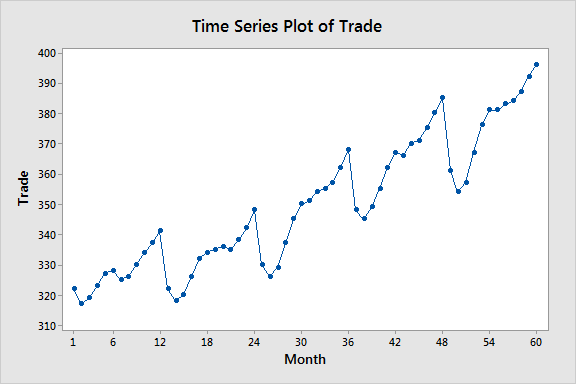
\includegraphics[scale=0.5]{img/ts-1}

Розглянемо наступний часовий ряд:

\begin{lstlisting}
import pandas as pd

data = pd.read_csv('../resources/sales.csv')
display(data.head(10))

# data = data.drop('Unnamed: 0', axis=1)
data.hist()
\end{lstlisting}

Результат:

\begin{console}
Unnamed: 0	Date	Sales
0	0	2021-10-01	29.109547
1	1	2021-10-02	30.720435
2	2	2021-10-03	30.305173
3	3	2021-10-04	27.390893
4	4	2021-10-05	22.841123
5	5	2021-10-06	19.002444
6	6	2021-10-07	23.904594
7	7	2021-10-08	27.544137
8	8	2021-10-09	30.567059
9	9	2021-10-10	30.087033
\end{console}

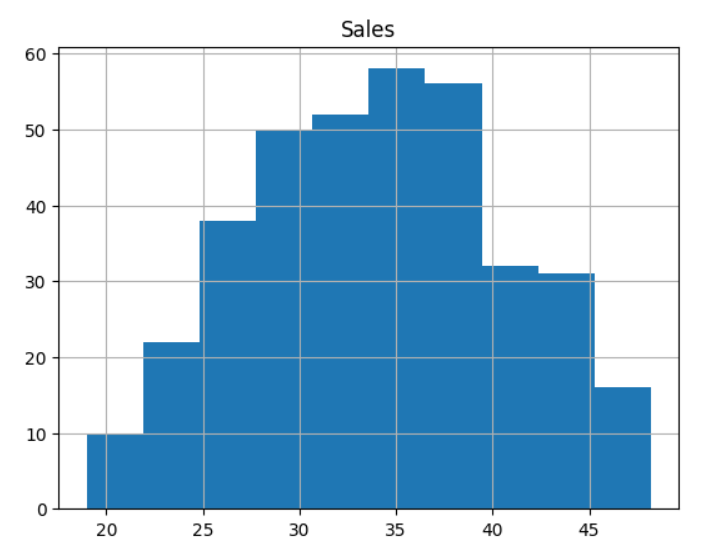
\includegraphics[scale=0.5]{img/208-1}

Зобразимо даний часовий ряд:

\begin{lstlisting}
data.plot(x='Date', y='Sales', kind='line', title='Daily Sales Over Time', figsize=(14, 5))
\end{lstlisting}

Результат:

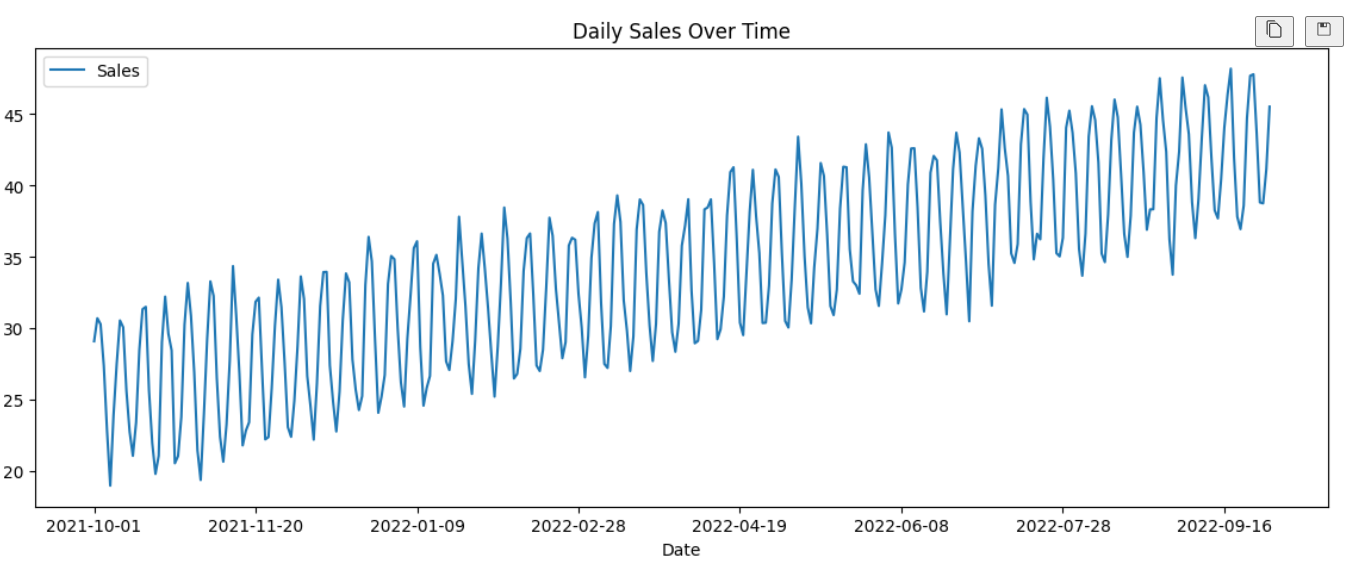
\includegraphics[scale=0.5]{img/208-2}

Виведемо, якільки є відсутніх даних:

\begin{lstlisting}
# data has no missing values
print(data.describe())
print("NAN values:",data.isna().sum())
\end{lstlisting}

Результат:

\begin{console}
            Sales
count  365.000000
mean    34.093942
std      6.572683
min     19.002444
25%     29.290376
50%     33.971567
75%     38.647294
max     48.190967
NAN values: Date     0
Sales    0
dtype: int64
\end{console}

На графіку вище чітко видно сезонну закономірність, яка повторюється тиждня, та висхідний тренд. Давайте детальніше розглянемо тренд та сезонну закономірність:

Шум (resid) - це часовий ряд після прибирання з нього тренду та сезонності. Це випадкові коливання значень, які не можна пояснити трендом, сезонністю або циклічністю. Причинами шуму можуть бути випадкові події або похибки у вимірюваннях. Шум не містить корисної закономірності та ускладнює аналіз даних - чим більший рівень шуму, тим складніше моделі знайти справжні закономірності.

\begin{lstlisting}
data['Date'] = pd.to_datetime(data['Date'])
data = data.set_index('Date')
data = data.asfreq('D')

from statsmodels.tsa.seasonal import seasonal_decompose

decomposed = seasonal_decompose(data['Sales']) 
decomposed.plot()
\end{lstlisting}

Результат:

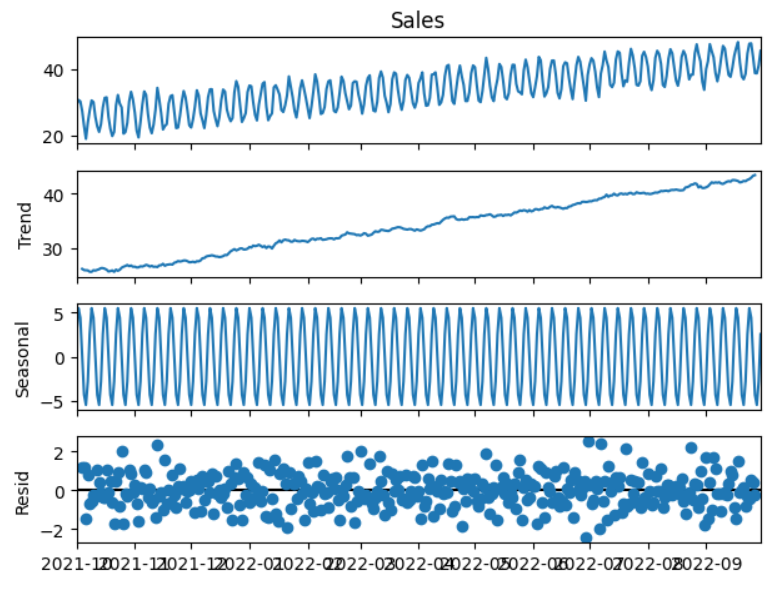
\includegraphics[scale=0.5]{img/208-3}


Диференціювання — це метод перетворення часового ряду, при якому кожне нове значення замінюється різницею між поточним і попереднім значенням. За допомогою диференціювання багато часових рядів можна зробити стаціонарними.


\subsection{Доповнений тест Дікі - Фуллера (ADF).}

Тест ADF - це тест для перевірки стаціонарності часового ряду на основі unit root - це процес, який через диференціювання визначає чи є часовий ряд стаціонарним. Тест працює за принципом приймання або відкидання нульової гіпотези, яка полягає у тому, що ряд не є стаціонарним. Приймати чи відкидати нульову гіпотезу вирішується за значенням p (вірогідність неправильності нульової гіпотези): якщо значення є більшим за визначену константу, то нульова гіпотеза приймається (ряд не є стаціонарним), якщо меншим - гіпотеза відкидається (ряд є стаціонарним). Традиційно, константа = 0.05 (5%), але може бути іншою, в залежності від даних та моделі.  Також важливо дивитися і на значення статистики, якщо воно більше за будь-яке критичне значення, то часовий ряд не є стаціонарним.

Розглянемо приклад дослідження числового ряду на стаціонарність за допомогою доповненого теста Дікі - Фуллера. Ми застосовуватимо можливості модуля statsmodels в python.

\begin{lstlisting}
from statsmodels.tsa.stattools import adfuller
import matplotlib.pyplot as plt

# data = data.drop('Unnamed: 0', axis=1)

def adfuller_test(df):
    adf=adfuller(df)
    statistic= adf[0]
    p_value=adf[1]
    critical_values=adf[4]
    return p_value,statistic,critical_values

def stat_check(df,p_value_check=0.05):
    movingAverage = df.rolling(window=12).mean()
    movingSTD = df.rolling(window=12).std()
    orig = plt.plot(df, color='blue', label='Original')
    mean = plt.plot(movingAverage, color='red', label='Rolling Mean')
    std = plt.plot(movingSTD, color='black', label='Rolling Std')
    plt.legend(loc='best')
    plt.title('Rolling Mean & Standard Deviation')
    plt.show(block=False)
    
    p_value,statistic,critical_values=adfuller_test(df)
    if (p_value<p_value_check):
        print('Time series is stationary, p value:{}'.format(p_value))
    else:
        print('Time series is NOT stationary, p value:{}'.format(p_value))
    print('Statistic:{}'.format(statistic))
    for key, value in critical_values.items():
        print('Critial Values:')
        print(f'   {key}, {value}')

stat_check(data)
\end{lstlisting}

Результат:

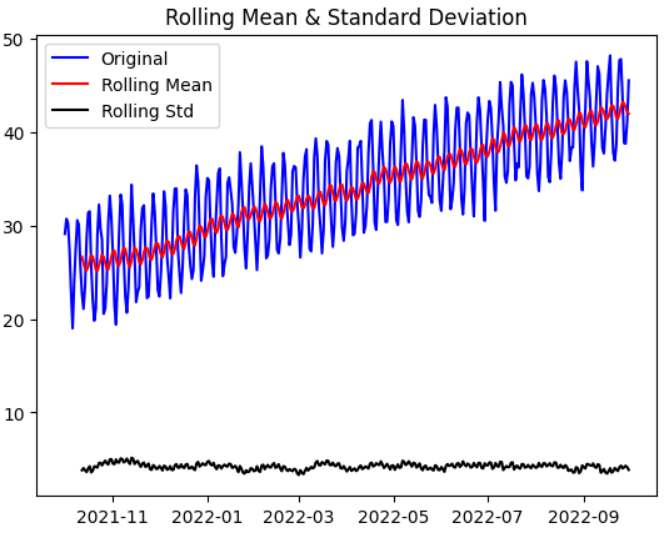
\includegraphics[scale=0.5]{img/208-4}


\begin{console}
Time series is NOT stationary, p value:0.979126294138459
Statistic:0.34045531718527483
Critial Values:
   1%, -3.4492815848836296
Critial Values:
   5%, -2.8698813715275406
Critial Values:
   10%, -2.5712138845950587
\end{console}

p-value показує ймовірність отримати спостережувані результати за умови, що нульова гіпотеза є істинною. Якщо p-value $< 0,05$, нульову гіпотезу відхиляють, і часовий ряд вважають стаціонарним; якщо p-value $\geq 0,05$, немає достатніх підстав відхилити нульову гіпотезу, тому ряд вважають нестаціонарним. Тест Дікі—Фуллера зазвичай виконують перед побудовою моделей ARIMA.



\section{Автокореляція.}

Кореляція - це зв’язок змінних між собою, автокореляція - зв’язок змінної з власними попередніми значенням. Оскільки ряд має тільки одну змінну, аналізувати потрібно тільки автокореляцію. Перед тим, як графік автокореляції розкриється у всій красі, розкажу про поняття lags (лаги) - це значення змінної n - кількість часу назад, оскільки розмірністю нашого часового ряду є день, то lag -1 означає значення 1 днів тому для поточної змінної, -2 -  два дні тому, тощо. На наведеному нижче графіку кількість лагів дорівнює 10.

\begin{lstlisting}
from statsmodels.graphics.tsaplots import plot_acf

plot_acf(data,lags=10)
plt.show()
\end{lstlisting}

Результат:

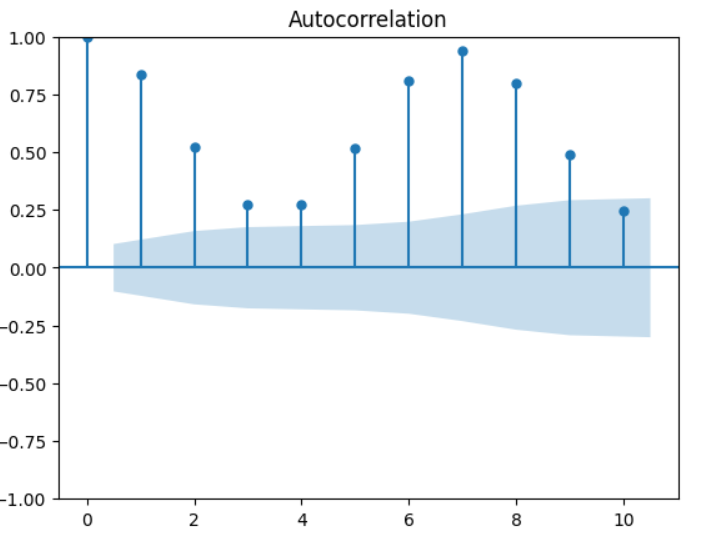
\includegraphics[scale=0.5]{img/208-5}

Декомпозиція - це процес перетворення нестаціонарного часового ряду у стаціонарний шляхом прибирання з нього сезонності та тренду.

Реконструкція часового ряду - це процес зворотнього додавання до ряду тренду та сезонності, якщо цього не зробити, ряд буде паралельним осі х та буде мало корисним як прогнозування.



\section{Функції втрати.}

Показниками якості моделей та прогнозування для часових рядів є функції втрати та метрики похибки. Найчастіше використовують такі функції втрати як MAE (L1 norm) - "Mean Square Error", MSE(L2 norm) - "Mean Absolute Error". 

\textbf{MAE} надає кожній помилці однакову"“вагу", тобто є робастною до викидів та шуму функцією, але одночасно з цим занижує "вплив" великих помилок.

Формула:

$$MAE = \frac{1}{n}\sum_{i=1}^{n}|y_{i} - \hat{y}_{i}|$$

\textbf{MSE} в свою чергу навпаки, дає більшим помилкам більшу вагу, що робить функцію більш чутливою до викидів. Якщо модель повинна бути чутлива до помилок, обирають саме цю функцію. 

Формула:

$$MSE = \frac{1}{n}\sum_{i=1}^{n}(y_{i} - \hat{y}_{i})^{2}$$

\textbf{Root Mean Squared Error} (RMSE) є квадратним коренем із середньої квадратичної помилки. Ця метрика також сильніше реагує на великі помилки, однак її перевага полягає в тому, що вона вимірюється в тих самих одиницях, що й прогнозований показник. Саме тому RMSE широко використовується для порівняння моделей прогнозування часових рядів.

Формула:

$$RMSE = \sqrt{\frac{1}{n}\sum_{i=1}^{n}(y_{i} - \hat{y}_{i})^{2}}$$

\textbf{Mean Absolute Percentage Error} (MAPE) або середня абсолютна відносна помилка показує середню величину помилки у відсотках. Наприклад, якщо MAPE дорівнює 5 $\%$, це означає, що прогноз у середньому відхиляється від реальних значень на п'ять відсотків. Завдяки такому представленню результати легко інтерпретувати та порівнювати між різними наборами даних. Водночас MAPE не рекомендується використовувати, якщо реальні значення можуть наближатися до нуля.

Формула:

$$MAPE = \frac{1}{n}\sum_{i=1}^{n}|\frac{y_{1} - \hat{y}_{i}}{y_{i}}|$$

\begin{lstlisting}
import numpy as np

def calculate_mape(actual, predicted): 
  
    if([isinstance(actual, np.ndarray) or isinstance(predicted, np.ndarray)]): 
        actual, predicted = np.array(actual),  np.array(predicted) 
    else:
        actual, predicted = np.Int(actual),  np.Int(predicted)
        
    return round(np.mean(np.abs(( 
      actual - predicted) / actual)) * 100, 2) 
\end{lstlisting}


\section{ARIMA.}

ARIMA (AutoRegressive Integrated Moving Average) — один із найпопулярніших методів класичного прогнозування часових рядів.
Його використовують, коли дані мають автокореляцію, тренд, але не обов’язково мають сезонність.

ARIMA дозволяє моделювати складні часові залежності й робити прогноз на майбутні значення.

Модель ARIMA описується трійкою параметрів:

$$ARIMA(p, d, q)$$

де p – кількість авторегресивних лагів (AR, або іншими словами, кількість попередніх значень), d – порядок диференціювання (I, Integrated) щоб зробити ряд стаціонарним, q – порядок ковзного середнього (MA, кількість попередніх похибок).

Поточне значення залежить від попередніх:

$$ y_t = \phi_1 y_{t-1} + \phi_2 y_{t-2} + \cdots + \phi_p y_{t-p} + \varepsilon_t $$

Авторегресійна частина (AR(p)) - поточне значення залежить від попередніх. Інтегрована частина (I(d)) - диференціювання робить ряд стаціонарним:

$$ y^{d}_t = y_t - y_{t-1} $$

або для d>1 – повторюється кілька разів. Стаціонарність важлива, бо AR і MA працюють саме з нею.

Ковзне середнє (MA(q)):

$$ y_t = \theta_1 \varepsilon_{t-1} + \theta_2 \varepsilon_{t-2} + \cdots + \theta_q \varepsilon_{t-q} + \varepsilon_t $$

Це модель залежності від попередніх випадкових шоків (помилок).

Повна модель ARIMA - поєднання всіх частин:

$$ ARIMA(p,d,q) = AR(p) + I(d) + MA(q) $$

Після диференціювання:

$$
y'_t = \phi_1 y'_{t-1} + ... + \phi_p y'_{t-p} +
\theta_1 \varepsilon_{t-1} + ... + \theta_q \varepsilon_{t-q} + \varepsilon_t
$$

Починаємо із $y'_{0} = y_{0}$

\begin{lstlisting}
from statsmodels.tsa.arima.model import ARIMA

model = ARIMA(data['Sales'], order=(7,1,7))
model_fit = model.fit()

print(model_fit.summary())
forecast = model_fit.forecast(steps=30)

print("Forecasted values:")
print(forecast)

plt.figure(figsize=(14, 5))
plt.plot(data['Sales'], label="Original Series")
plt.plot(forecast.index, forecast, label="Forecast", linestyle='--')
plt.legend()
plt.title("ARIMA Forecast Example")
plt.show()
\end{lstlisting}

Результат:

\begin{console}
                               SARIMAX Results                                
==============================================================================
Dep. Variable:                  Sales   No. Observations:                  365
Model:                 ARIMA(7, 1, 7)   Log Likelihood                -536.758
Date:                Fri, 21 Nov 2025   AIC                           1103.517
Time:                        12:02:09   BIC                           1161.974
Sample:                    10-01-2021   HQIC                          1126.751
                         - 09-30-2022                                         
Covariance Type:                  opg                                         
==============================================================================
                 coef    std err          z      P>|z|      [0.025      0.975]
------------------------------------------------------------------------------
ar.L1         -1.5086      1.264     -1.193      0.233      -3.986       0.969
ar.L2         -1.0640      0.866     -1.228      0.219      -2.762       0.634
ar.L3         -0.8506      0.554     -1.536      0.124      -1.936       0.235
ar.L4         -1.3599      0.572     -2.376      0.018      -2.482      -0.238
ar.L5         -1.4469      1.224     -1.182      0.237      -3.846       0.952
ar.L6         -0.7478      0.760     -0.984      0.325      -2.238       0.742
ar.L7         -0.1451      0.231     -0.629      0.529      -0.597       0.307
ma.L1          0.5698      1.260      0.452      0.651      -1.900       3.039
ma.L2         -0.2415      0.583     -0.414      0.679      -1.385       0.902
ma.L3          0.0016      0.369      0.004      0.997      -0.721       0.724
ma.L4          0.6490      0.221      2.934      0.003       0.216       1.083
ma.L5          0.3343      0.746      0.448      0.654      -1.129       1.797
ma.L6         -0.4259      0.335     -1.270      0.204      -1.083       0.232
ma.L7         -0.3330      0.435     -0.765      0.444      -1.186       0.520
sigma2         1.1157      0.091     12.310      0.000       0.938       1.293
===================================================================================
Ljung-Box (L1) (Q):                   0.00   Jarque-Bera (JB):                 0.39
Prob(Q):                              0.95   Prob(JB):                         0.82
Heteroskedasticity (H):               0.92   Skew:                             0.08
Prob(H) (two-sided):                  0.67   Kurtosis:                         3.02
===================================================================================

Warnings:
[1] Covariance matrix calculated using the outer product of gradients (complex-step).
Forecasted values:
2022-10-01    48.616060
2022-10-02    47.693508
2022-10-03    43.710640
2022-10-04    39.170891
2022-10-05    37.856026
2022-10-06    40.696951
2022-10-07    45.373877
2022-10-08    48.592830
2022-10-09    47.813319
2022-10-10    43.598087
2022-10-11    39.219554
2022-10-12    37.894455
2022-10-13    40.630354
2022-10-14    45.411763
2022-10-15    48.584311
2022-10-16    47.786612
2022-10-17    43.630119
2022-10-18    39.215936
2022-10-19    37.889536
2022-10-20    40.644359
2022-10-21    45.394903
2022-10-22    48.578806
2022-10-23    47.792791
2022-10-24    43.627127
2022-10-25    39.225426
2022-10-26    37.895271
2022-10-27    40.638293
2022-10-28    45.391572
2022-10-29    48.573010
2022-10-30    47.790048
Freq: D, Name: predicted_mean, dtype: float64
\end{console}

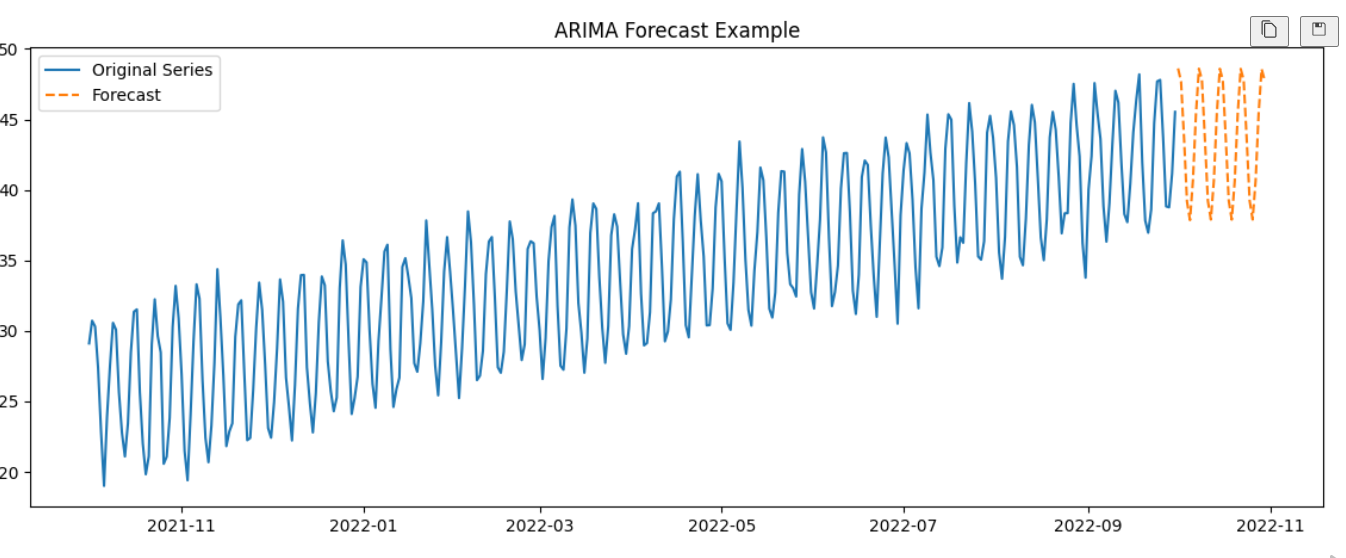
\includegraphics[scale=0.5]{img/208-6}

\ding{43} ARIMA доцільно використовувати, якщо часовий ряд є стаціонарним або його можна зробити стаціонарним за допомогою диференціювання. ARIMA підходить також для часових рядів що не мають складних нелінійних залежностей. 

Проте ARIMA звісно має свої обмеження із моделюванням нелінійних залежностей. Точність для стаціонарних рядів без нелінійних залежностей, точність для довгострокового прогнозування стрімко падає. 

Якщо часовий ряд має складну структуру або залежить від багатьох факторів, часто ефективнішими є методи машинного навчання або глибокого навчання.


\section{Передбачення із використанням методів машинного навчання.}

Застосуємо ансамблеву модель випадкового лісу для передбачення значення часового ряду. Тут ознаками будуть лагові значення (попередні $n$ значень часового ряду), цільовою змінною буде поточне значення, яке потрібно передбачити. Таким чином модель навчається прогнозувати наступне значення за кількома попередніми.

\begin{lstlisting}
import numpy as np
import pandas as pd
import matplotlib.pyplot as plt
from sklearn.ensemble import RandomForestRegressor

def create_lags(series, n_lags=10):
    df = pd.DataFrame({"y": series})
    for i in range(1, n_lags + 1):
        df[f"lag_{i}"] = df["y"].shift(i)
    return df.dropna()

N_LAGS = 10
df_lags = create_lags(data['Sales'], N_LAGS)

X = df_lags.drop("y", axis=1)
y = df_lags["y"]

model = RandomForestRegressor(n_estimators=500, random_state=42)
model.fit(X, y)

steps = 30
last_values = list(data['Sales'].values[-N_LAGS:])
forecast_values = []

for _ in range(steps):
    x_input = np.array(last_values[-N_LAGS:]).reshape(1, -1)
    y_pred = model.predict(x_input)[0]
    
    forecast_values.append(y_pred)
    last_values.append(y_pred)

last_date = data.index[-1]
future_index = pd.date_range(start=last_date, periods=steps+1, freq='D')[1:]

forecast = pd.Series(forecast_values, index=future_index)

print("Forecast:")
plt.figure(figsize=(14, 5))
plt.plot(data['Sales'], label="Original Series")
plt.plot(forecast.index, forecast, label="Random Forest Forecast", linestyle='--')
plt.legend()
plt.title("Random Forest Forecast with Lag Features")
plt.show()
\end{lstlisting}

Результат:

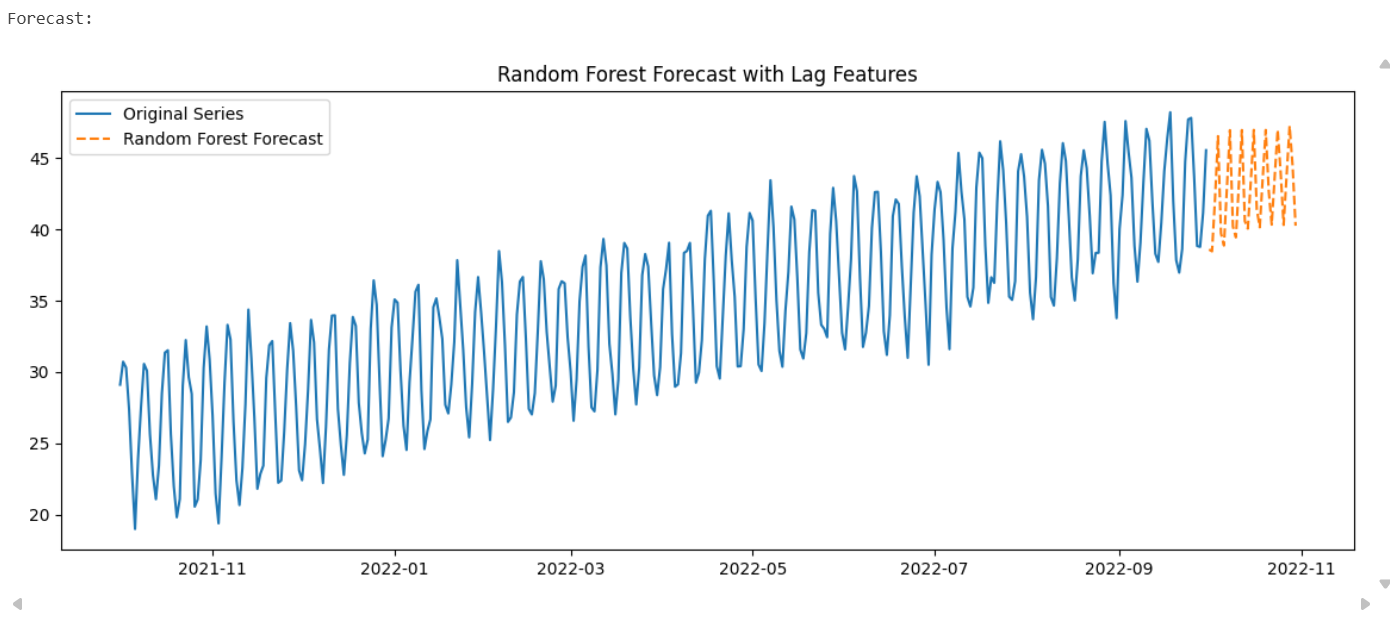
\includegraphics[scale=0.5]{img/208-7}

Для задач із великою кількістю даних і складними закономірностями найкращі результати часто демонструють LSTM, GRU та Transformer-моделі.

У звичайних задачах машинного навчання випадкове перемішування даних допомагає уникнути зміщення вибірки. Для часових рядів цього робити не можна, оскільки спостереження мають природний часовий порядок. Якщо випадково перемішати дані, модель може отримати інформацію з майбутнього під час навчання, що призведе до так званого витоку даних (Data Leakage).

\section{Експоненційне зглажування.}

Експоненційне згладжування — це клас методів прогнозування часових рядів, у яких останні спостереження отримують більшу вагу, ніж старі.
Ваги зменшуються експоненційно, звідки й назва. Завдяки цьому модель швидше реагує на зміни в даних і водночас згладжує випадкові коливання. На відміну від простого ковзного середнього, ваги попередніх спостережень зменшуються експоненційно, що й дало назву цьому методу.

Нехай $ y_t $ — фактичне значення часового ряду, а $ \hat{y}_{t} $ — прогноз.

Тоді просте експоненційне згладжування (SES) визначається як:

$$
\hat{y}_{t} = \alpha y_{t-1} + (1 - \alpha)\hat{y}_{t-1}
$$

де $ 0 < \alpha < 1 $ — коефіцієнт згладжування, велике $ \alpha $ - модель сильніше реагує на нові дані, мале $ \alpha $ - прогноз згладжений, повільно змінюється

Експоненційне згладжування найкраще підходить для часових рядів, у яких зберігаються відносно стабільні закономірності. Просте згладжування використовується для стаціонарних рядів без тренду, метод Хольта — для рядів із трендом, а метод Хольта—Вінтерса — для даних, що містять як тренд, так і сезонність. Ці методи широко застосовуються для короткострокового прогнозування економічних показників, продажів, попиту на товари, споживання електроенергії та інших процесів.


\textbf{Модель Холта (Holt’s Linear Trend)}: якщо в ряді є тренд, ми додаємо окрему модель для тренду:

$$
\begin{aligned}
\hat{y}_{t} &= \ell_{t-1} + b_{t-1} \
\ell_t &= \alpha y_t + (1-\alpha)(\ell_{t-1} + b_{t-1}) \
b_t &= \beta (\ell_t - \ell_{t-1}) + (1-\beta) b_{t-1}
\end{aligned}
$$

де $ \ell_t $ — рівень, $ b_t $ — тренд, $ \alpha, \beta \in (0,1) $

\begin{lstlisting}
import matplotlib.pyplot as plt
from statsmodels.tsa.holtwinters import ExponentialSmoothing

model = ExponentialSmoothing(
    data['Sales'],
    trend="add",      
    seasonal=None     
)

model_fit = model.fit()
forecast = model_fit.forecast(30)

print("Forecast:")
plt.figure(figsize=(10, 5))
plt.plot(data['Sales'], label="Original Series")
plt.plot(forecast.index, forecast, label="Exponential Smoothing Forecast", linestyle="--")
plt.legend()
plt.title("Exponential Smoothing Forecast Example")
plt.show()
\end{lstlisting}

Результат:

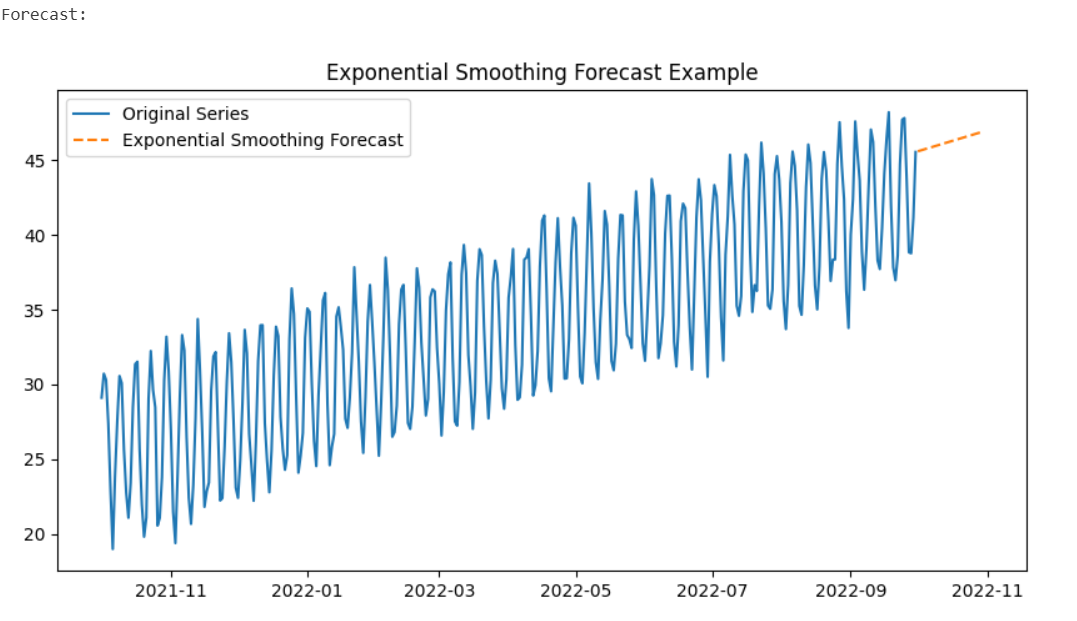
\includegraphics[scale=0.5]{img/208-8}

\ding{43} Варто пам'ятати, що методи машинного навчання потребують значно більшої кількості навчальних даних для правильного прогнозу. Окрім того, вони часто є менш інтерпретованими, та мають високу обчислювальну складність. У сучасному інтелектуальному аналізі даних вибір моделі залежить від конкретної задачі. Для невеликих і добре структурованих часових рядів часто достатньо моделей ARIMA або експоненційного згладжування. Якщо ж часовий ряд має складні нелінійні залежності або залежить від великої кількості зовнішніх факторів, доцільніше використовувати методи машинного навчання чи глибокого навчання, такі як XGBoost, LSTM або Transformer.



\ding{46} \textbf{Питання для самоконтролю.}

\begin{enumerate}
\item Що таке часовий ряд?
\item Чим часовий ряд відрізняється від звичайного набору даних?
\item Які приклади часових рядів можна зустріти в інтелектуальному аналізі даних?
\item Які основні компоненти містить часовий ряд?
\item Що таке тренд у часовому ряді?
\item Що таке сезонність?
\item Що таке шум у часовому ряді?
\item Як шум впливає на точність прогнозування?
\item Що таке стаціонарний часовий ряд?
\item Чому стаціонарність є важливою під час побудови моделей прогнозування?
\item Які характеристики стаціонарного часового ряду залишаються незмінними з часом?
\item Як можна перетворити нестаціонарний часовий ряд на стаціонарний?
\item Що таке диференціювання (Differencing)?
\item Для чого використовується тест Дікі—Фуллера (Augmented Dickey–Fuller Test)?
\item Як інтерпретувати результати тесту Дікі—Фуллера?
\item Що означає p-value у тесті Дікі—Фуллера?
\item Що таке автокореляція?
\item Як автокореляція використовується під час аналізу часових рядів?
\item Що показує функція автокореляції (ACF)?
\item Для чого використовується часткова автокореляційна функція (PACF)?
\item Яку роль відіграють графіки ACF та PACF при виборі параметрів моделі ARIMA?
\item Що таке модель ARIMA?
\item Що означають параметри p, d та q у моделі ARIMA?
\item У яких випадках доцільно використовувати модель ARIMA?
\item Які обмеження має модель ARIMA?
\item Що таке експоненційне згладжування?
\item Чим просте експоненційне згладжування відрізняється від методів Хольта та Хольта—Вінтерса?
\item Для яких часових рядів найкраще підходить експоненційне згладжування?
\item Які функції втрат використовуються для оцінювання якості прогнозування часових рядів?
\item Що таке Mean Absolute Error (MAE)?
\item Що таке Mean Squared Error (MSE)?
\item Що таке Root Mean Squared Error (RMSE)?
\item Що таке Mean Absolute Percentage Error (MAPE)?
\item Чому для прогнозування часових рядів застосовують методи машинного навчання?
\item Які алгоритми машинного навчання найчастіше використовуються для прогнозування часових рядів?
\item Як формується навчальна вибірка для моделей машинного навчання при роботі з часовими рядами?
\item Чому під час прогнозування часових рядів не можна випадково перемішувати дані перед навчанням моделі?
\item Які переваги та недоліки мають класичні статистичні моделі (ARIMA, експоненційне згладжування) порівняно з сучасними методами машинного навчання?
\end{enumerate}
